\documentclass[]{book}
\usepackage{lmodern}
\usepackage{amssymb,amsmath}
\usepackage{ifxetex,ifluatex}
\usepackage{fixltx2e} % provides \textsubscript
\ifnum 0\ifxetex 1\fi\ifluatex 1\fi=0 % if pdftex
  \usepackage[T1]{fontenc}
  \usepackage[utf8]{inputenc}
\else % if luatex or xelatex
  \ifxetex
    \usepackage{mathspec}
  \else
    \usepackage{fontspec}
  \fi
  \defaultfontfeatures{Ligatures=TeX,Scale=MatchLowercase}
\fi
% use upquote if available, for straight quotes in verbatim environments
\IfFileExists{upquote.sty}{\usepackage{upquote}}{}
% use microtype if available
\IfFileExists{microtype.sty}{%
\usepackage{microtype}
\UseMicrotypeSet[protrusion]{basicmath} % disable protrusion for tt fonts
}{}
\usepackage[margin=1in]{geometry}
\usepackage{hyperref}
\hypersetup{unicode=true,
            pdftitle={Analisis Bisinis Menggunakan R},
            pdfauthor={Aep Hidayatuloh},
            pdfborder={0 0 0},
            breaklinks=true}
\urlstyle{same}  % don't use monospace font for urls
\usepackage{natbib}
\bibliographystyle{apalike}
\usepackage{color}
\usepackage{fancyvrb}
\newcommand{\VerbBar}{|}
\newcommand{\VERB}{\Verb[commandchars=\\\{\}]}
\DefineVerbatimEnvironment{Highlighting}{Verbatim}{commandchars=\\\{\}}
% Add ',fontsize=\small' for more characters per line
\usepackage{framed}
\definecolor{shadecolor}{RGB}{248,248,248}
\newenvironment{Shaded}{\begin{snugshade}}{\end{snugshade}}
\newcommand{\AlertTok}[1]{\textcolor[rgb]{0.94,0.16,0.16}{#1}}
\newcommand{\AnnotationTok}[1]{\textcolor[rgb]{0.56,0.35,0.01}{\textbf{\textit{#1}}}}
\newcommand{\AttributeTok}[1]{\textcolor[rgb]{0.77,0.63,0.00}{#1}}
\newcommand{\BaseNTok}[1]{\textcolor[rgb]{0.00,0.00,0.81}{#1}}
\newcommand{\BuiltInTok}[1]{#1}
\newcommand{\CharTok}[1]{\textcolor[rgb]{0.31,0.60,0.02}{#1}}
\newcommand{\CommentTok}[1]{\textcolor[rgb]{0.56,0.35,0.01}{\textit{#1}}}
\newcommand{\CommentVarTok}[1]{\textcolor[rgb]{0.56,0.35,0.01}{\textbf{\textit{#1}}}}
\newcommand{\ConstantTok}[1]{\textcolor[rgb]{0.00,0.00,0.00}{#1}}
\newcommand{\ControlFlowTok}[1]{\textcolor[rgb]{0.13,0.29,0.53}{\textbf{#1}}}
\newcommand{\DataTypeTok}[1]{\textcolor[rgb]{0.13,0.29,0.53}{#1}}
\newcommand{\DecValTok}[1]{\textcolor[rgb]{0.00,0.00,0.81}{#1}}
\newcommand{\DocumentationTok}[1]{\textcolor[rgb]{0.56,0.35,0.01}{\textbf{\textit{#1}}}}
\newcommand{\ErrorTok}[1]{\textcolor[rgb]{0.64,0.00,0.00}{\textbf{#1}}}
\newcommand{\ExtensionTok}[1]{#1}
\newcommand{\FloatTok}[1]{\textcolor[rgb]{0.00,0.00,0.81}{#1}}
\newcommand{\FunctionTok}[1]{\textcolor[rgb]{0.00,0.00,0.00}{#1}}
\newcommand{\ImportTok}[1]{#1}
\newcommand{\InformationTok}[1]{\textcolor[rgb]{0.56,0.35,0.01}{\textbf{\textit{#1}}}}
\newcommand{\KeywordTok}[1]{\textcolor[rgb]{0.13,0.29,0.53}{\textbf{#1}}}
\newcommand{\NormalTok}[1]{#1}
\newcommand{\OperatorTok}[1]{\textcolor[rgb]{0.81,0.36,0.00}{\textbf{#1}}}
\newcommand{\OtherTok}[1]{\textcolor[rgb]{0.56,0.35,0.01}{#1}}
\newcommand{\PreprocessorTok}[1]{\textcolor[rgb]{0.56,0.35,0.01}{\textit{#1}}}
\newcommand{\RegionMarkerTok}[1]{#1}
\newcommand{\SpecialCharTok}[1]{\textcolor[rgb]{0.00,0.00,0.00}{#1}}
\newcommand{\SpecialStringTok}[1]{\textcolor[rgb]{0.31,0.60,0.02}{#1}}
\newcommand{\StringTok}[1]{\textcolor[rgb]{0.31,0.60,0.02}{#1}}
\newcommand{\VariableTok}[1]{\textcolor[rgb]{0.00,0.00,0.00}{#1}}
\newcommand{\VerbatimStringTok}[1]{\textcolor[rgb]{0.31,0.60,0.02}{#1}}
\newcommand{\WarningTok}[1]{\textcolor[rgb]{0.56,0.35,0.01}{\textbf{\textit{#1}}}}
\usepackage{longtable,booktabs}
\usepackage{graphicx,grffile}
\makeatletter
\def\maxwidth{\ifdim\Gin@nat@width>\linewidth\linewidth\else\Gin@nat@width\fi}
\def\maxheight{\ifdim\Gin@nat@height>\textheight\textheight\else\Gin@nat@height\fi}
\makeatother
% Scale images if necessary, so that they will not overflow the page
% margins by default, and it is still possible to overwrite the defaults
% using explicit options in \includegraphics[width, height, ...]{}
\setkeys{Gin}{width=\maxwidth,height=\maxheight,keepaspectratio}
\IfFileExists{parskip.sty}{%
\usepackage{parskip}
}{% else
\setlength{\parindent}{0pt}
\setlength{\parskip}{6pt plus 2pt minus 1pt}
}
\setlength{\emergencystretch}{3em}  % prevent overfull lines
\providecommand{\tightlist}{%
  \setlength{\itemsep}{0pt}\setlength{\parskip}{0pt}}
\setcounter{secnumdepth}{5}
% Redefines (sub)paragraphs to behave more like sections
\ifx\paragraph\undefined\else
\let\oldparagraph\paragraph
\renewcommand{\paragraph}[1]{\oldparagraph{#1}\mbox{}}
\fi
\ifx\subparagraph\undefined\else
\let\oldsubparagraph\subparagraph
\renewcommand{\subparagraph}[1]{\oldsubparagraph{#1}\mbox{}}
\fi

%%% Use protect on footnotes to avoid problems with footnotes in titles
\let\rmarkdownfootnote\footnote%
\def\footnote{\protect\rmarkdownfootnote}

%%% Change title format to be more compact
\usepackage{titling}

% Create subtitle command for use in maketitle
\providecommand{\subtitle}[1]{
  \posttitle{
    \begin{center}\large#1\end{center}
    }
}

\setlength{\droptitle}{-2em}

  \title{Analisis Bisinis Menggunakan R}
    \pretitle{\vspace{\droptitle}\centering\huge}
  \posttitle{\par}
    \author{Aep Hidayatuloh}
    \preauthor{\centering\large\emph}
  \postauthor{\par}
    \date{}
    \predate{}\postdate{}
  
\usepackage{booktabs}

\begin{document}
\maketitle

{
\setcounter{tocdepth}{1}
\tableofcontents
}
\hypertarget{kata-pengantar}{%
\chapter*{Kata Pengantar}\label{kata-pengantar}}
\addcontentsline{toc}{chapter}{Kata Pengantar}

\emph{Assalamu 'alaikum warohmatullohi wabarokatuh\ldots{}}

\emph{Alhamdulillahi robbil'alamiin\ldots{}}

Segala puji dan syukur hanya untuk Alloh Subhanahu Wa Ta'ala karena atas rahmat dan ridho-Nya buku ini dapat diselesaikan. Buku ini ditulis untuk menuangkan ide dan pengalaman melakukan penelitian di beberapa bidang bisnis sebagai konsultan analisis data maupun karyawan di sebuah perusahaan.

Buku ini disusun dengan menggunakan R versi 3.6.0 64bit pada Windows 10, \textbf{RMarkdown} dan \textbf{bookdown}. Tujuan utama dari buku ini adalah untuk membantu yang ingin belajar analisis data menggunakan R melalui pendekatan bisnis. Contoh kasus yang disajikan diharapkan dapat memperdalam pemaham pembaca mengenai materi dan permasalahan bisnis yang dapat diselesaikan. Contoh script yang digunakan lebih banyak menggunakan \href{https://www.tidyverse.org/}{tidyverse}.

Dalam buku ini tidak akan dibahas secara detail dari suatu teori atau algoritma. Tidak juga akan membahas teori statistika yang digunakan. Di dalam buku ini lebih ditekankan pada penggunaan R sebagai tools untuk analisis data.

This is a \emph{simple} book written in \textbf{Markdown}. You can use anything that Pandoc's Markdown supports, e.g., a math equation \(a^2 + b^2 = c^2\).

The \textbf{bookdown} package can be installed from CRAN or Github:

\begin{Shaded}
\begin{Highlighting}[]
\KeywordTok{install.packages}\NormalTok{(}\StringTok{"bookdown"}\NormalTok{)}
\CommentTok{# or the development version}
\CommentTok{# devtools::install_github("rstudio/bookdown")}
\end{Highlighting}
\end{Shaded}

Remember each Rmd file contains one and only one chapter, and a chapter is defined by the first-level heading \texttt{\#}.

To compile this example to PDF, you need XeLaTeX. You are recommended to install TinyTeX (which includes XeLaTeX): \url{https://yihui.name/tinytex/}.

\hypertarget{business}{%
\chapter{Bisinis dan Data-Driven}\label{business}}

Membahas tentang Bisnis dan perkembangannya di masa sebelum dan setelah perkembangan analisis data.

\hypertarget{analisis-data-dan-bisnis}{%
\section{Analisis Data dan Bisnis}\label{analisis-data-dan-bisnis}}

Kebutuhan terhadap analis data (\emph{data analyst}) meningkat begitu pesat dalam beberapa tahun terakhir ini. Hal ini karena para pengambil keputusan mulai menyadari pentingnya bisnis berdasarkan data agar dapat bertahan dalam kompetisi yang sangat ketat. Analisis adalah penggunaan data, teknologi informasi, statistika, metode kuantitatif dan model matematika atau \emph{computer-based}.

Penggunaan analisis data untuk meningkatkan perkembangan bisnis sudah tidak diragukan lagi. Banyak perusahaan, terutama yang berbasis teknologi informasi atau perintis (\emph{startup}), menjadikan analisis data sebagai fondasi utama bisnis mereka. Bisnis yang dijalankan mengkolaborasikan antara pengetahuan bisnis dan analisis data sehingga menghasilkan keuntungan yang sangat tinggi.

Perusahaan seperti ini tidak lagi hanya menjadikan intuisi atau pengalaman senior-senior di perusahaan tersebut sebagai pijakan utama. Bahkan sebagian besar dari pegawai perusahaan tersebut adalah anak-anak muda yang jika dilihat dari pengalaman di dunia bisnis masih seumur jagung. Namun, mereka menyadari bahwa telah terjadi pergeseran perilaku konsumen dan menemukan kesempatan atau kebutuhan baru di pasar yang belum tersedia.

\hypertarget{penerapan-analisis-data}{%
\section{Penerapan Analisis Data}\label{penerapan-analisis-data}}

Setiap perusahaan harus bisa memetakan kebutuhan terhadap analisis data di perusahaannya. Jika penggunaan analisis data pada bagian yang tepat maka hal ini dapat memberian keuntungan yang tinggi atau menurunkan biaya produksi sehingga bisnis lebih optimal.

\hypertarget{customer-relationship-management-crm}{%
\subsection{Customer Relationship Management (CRM)}\label{customer-relationship-management-crm}}

Penggunana analisis data yang paling sering adalah CRM. Hampir semua bisnis saat ini menjadikan pelanggan dan pasar sebagai landasan dalam pengambilan keputusan. Berbeda dengan bisnis di jaman dulu, ketika perusahaanlah yang menentukan kondisi pasar, produk yang akan mereka jual atau jasa apa yang akan mereka berikan.

\hypertarget{finansial-dan-produk}{%
\subsection{Finansial dan Produk}\label{finansial-dan-produk}}

Analisis data dalam bidang finasial sudah banyak digunakan, terutama dalam bidang perbankan. Beberapa perusahaan juga menggunakan analisis data untuk menentukan kelayakan produk atau jasa yang mereka miliki, dan juga untuk melakukan pengembangan produk atau jasa.

\hypertarget{manajemen-rantai-pasokan}{%
\subsection{Manajemen Rantai Pasokan}\label{manajemen-rantai-pasokan}}

Manajemen Rantai Pasokan (\emph{Supply Chain Management}) yang baik sangat diperlukan oleh industri. Optimalisasi sumber daya yang ada agar dapat menjalankan bisnis dengan efektif, efisien dan memberikan keuntungan yang besar menjadi target utama.

\hypertarget{manajemen-sumber-daya-manusia}{%
\subsection{Manajemen Sumber Daya Manusia}\label{manajemen-sumber-daya-manusia}}

Bagian Manajemen Sumber Daya Manusia (\emph{Human Resources Management}) di sebuah perusahaan dapat memperkirakan dengan lebih baik jika ada karyawan yang ingin berhenti (\emph{churn}), meningkatkan prestasi karyawan, bahkan dapat mengetahui profil karyawan seperti apa yang cocok dan mempunyai peluang karir yang baik melalui analisis data.

\hypertarget{penentuan-harga}{%
\subsection{Penentuan Harga}\label{penentuan-harga}}

Penentuan harga (\emph{pricing decision}) dalam persaingan bisnis di era modern dan serba canggih ini sangat berpengaruh terhadap bisnis.

\hypertarget{rekomendasi-belanja}{%
\subsection{Rekomendasi Belanja}\label{rekomendasi-belanja}}

Ketika Anda belanja di sebuah \emph{e-commerce}, pasti akan selalu ada bagian yang menawarkan barang lain yang mungkin sedang Anda cari.

\hypertarget{startegi-tim-olahraga}{%
\subsection{Startegi Tim Olahraga}\label{startegi-tim-olahraga}}

Bukan hanya di dunia bisnis, analisis data sudah sejak lama digunakan untuk meningkatkan kemampuan dan kualitas sebuah tim olahraga. Anda pernah mendengar atau menonton sebuah film berjudul \href{https://www.google.com/search?safe=strict\&ei=JBjRXNC4Mpvaz7sP9ra30AQ\&q=moneyball\&oq=moneyball\&gs_l=psy-ab.3..0i67l2j0i7i30l2j0i67j0i7i30l5.24699.24699..25317...0.0..0.260.260.2-1......0....1..gws-wiz.......0i71.JqVXxSHAnjo}{\textbf{Moneyball}}? Ini adalah sebuah film yang dibuat berdasarkan kisah nyata. Seorang pelatih menjadikan seorang analis data sebagai asistennya dalam merekrut dan menempatkan atlit baseball berdasarkan hasil analisis data.

\hypertarget{investasi}{%
\section{Investasi}\label{investasi}}

Agar lingkungan analisis data dapat tercipta dan memberikan efek yang signifikan, perusahaan atau institusi bisnis harus mau berinvestasi dan mungkin butuh waktu yang cukup lama untuk melihat hasil dari sistem analisis data ini. Investasi yang \emph{--minimal--} harus dilakukan oleh perusahaan adalah:

\begin{enumerate}
\def\labelenumi{\arabic{enumi}.}
\tightlist
\item
  Memperbaiki sistem pencatatan dan pengumpulan data.
\item
  Menyediakan infrastruktur untuk menyimpan data.
\item
  Menyiapkan infrastruktur untuk lingkungan analisis data yang baik.
\item
  Evaluasi hasil.
\item
  Meningkatkan atau memperbaiki (\emph{improve}) sistem analisis data.
\end{enumerate}

Banyak institusi bisnis yang awalnya menggebu-gebu ingin menerapkan sistem analisis data, namun merasa enggan setelah mengetahui investasi yang dibutuhkan.

You can label chapter and section titles using \texttt{\{\#label\}} after them, e.g., we can reference Chapter \ref{business}. If you do not manually label them, there will be automatic labels anyway, e.g., Chapter \ref{intro}.

Figures and tables with captions will be placed in \texttt{figure} and \texttt{table} environments, respectively.

\begin{Shaded}
\begin{Highlighting}[]
\KeywordTok{par}\NormalTok{(}\DataTypeTok{mar =} \KeywordTok{c}\NormalTok{(}\DecValTok{4}\NormalTok{, }\DecValTok{4}\NormalTok{, }\FloatTok{.1}\NormalTok{, }\FloatTok{.1}\NormalTok{))}
\KeywordTok{plot}\NormalTok{(pressure, }\DataTypeTok{type =} \StringTok{'b'}\NormalTok{, }\DataTypeTok{pch =} \DecValTok{19}\NormalTok{)}
\end{Highlighting}
\end{Shaded}

\begin{figure}

{\centering 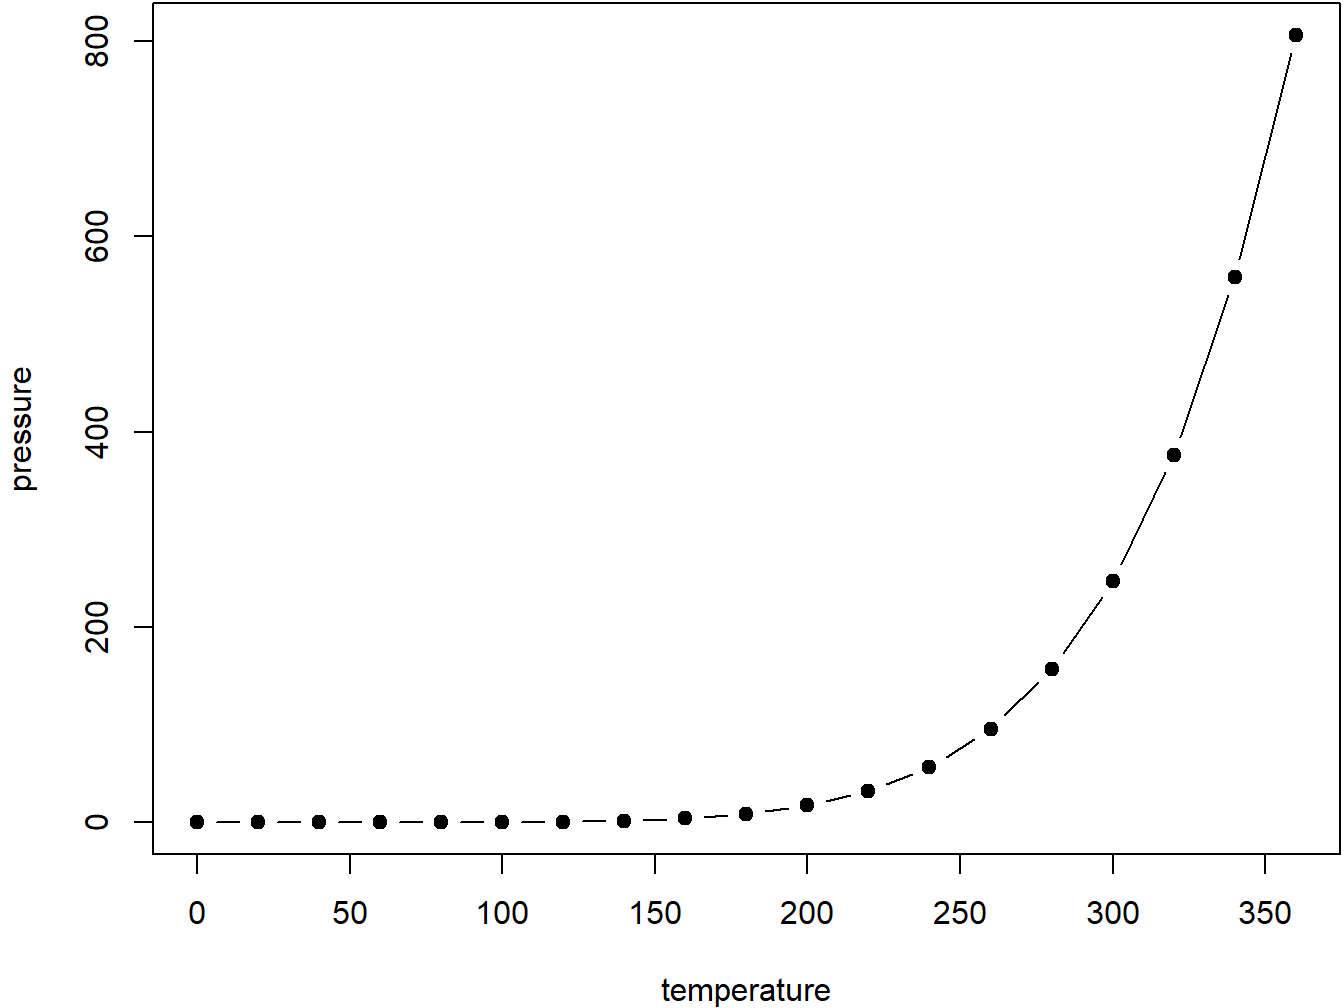
\includegraphics[width=0.8\linewidth]{buku_files/figure-latex/nice-fig-1} 

}

\caption{Here is a nice figure!}\label{fig:nice-fig}
\end{figure}

Reference a figure by its code chunk label with the \texttt{fig:} prefix, e.g., see Figure \ref{fig:nice-fig}. Similarly, you can reference tables generated from \texttt{knitr::kable()}, e.g., see Table \ref{tab:nice-tab}.

\begin{Shaded}
\begin{Highlighting}[]
\NormalTok{knitr}\OperatorTok{::}\KeywordTok{kable}\NormalTok{(}
  \KeywordTok{head}\NormalTok{(iris, }\DecValTok{10}\NormalTok{), }\DataTypeTok{caption =} \StringTok{'Here is a nice table!'}\NormalTok{,}
  \DataTypeTok{booktabs =} \OtherTok{TRUE}
\NormalTok{)}
\end{Highlighting}
\end{Shaded}

\begin{table}[t]

\caption{\label{tab:nice-tab}Here is a nice table!}
\centering
\begin{tabular}{rrrrl}
\toprule
Sepal.Length & Sepal.Width & Petal.Length & Petal.Width & Species\\
\midrule
5.1 & 3.5 & 1.4 & 0.2 & setosa\\
4.9 & 3.0 & 1.4 & 0.2 & setosa\\
4.7 & 3.2 & 1.3 & 0.2 & setosa\\
4.6 & 3.1 & 1.5 & 0.2 & setosa\\
5.0 & 3.6 & 1.4 & 0.2 & setosa\\
\addlinespace
5.4 & 3.9 & 1.7 & 0.4 & setosa\\
4.6 & 3.4 & 1.4 & 0.3 & setosa\\
5.0 & 3.4 & 1.5 & 0.2 & setosa\\
4.4 & 2.9 & 1.4 & 0.2 & setosa\\
4.9 & 3.1 & 1.5 & 0.1 & setosa\\
\bottomrule
\end{tabular}
\end{table}

You can write citations, too. For example, we are using the \textbf{bookdown} package \citep{xie2019} in this sample book, which was built on top of R Markdown and \textbf{knitr} \citep{xie2015}. \citep{hadley}

\hypertarget{intro}{%
\chapter{Pengantar R}\label{intro}}

\hypertarget{kenapa-memilih-r}{%
\section{Kenapa Memilih R?}\label{kenapa-memilih-r}}

R adalah sebuah program komputasi statistika dan grafis \citep{R-base}. Saat ini R sudah dikenal luas sebagai salah satu \emph{powerful software} untuk analisis data dan \emph{Data Science}. Tentu saja selain R masih banyak \emph{software} lain yang tidak kalah dengan R, misalnya Python. Berikut ini beberapa hal diantara kelebihan R.

\begin{enumerate}
\def\labelenumi{\arabic{enumi}.}
\tightlist
\item
  Gratis dan Open Source
\item
  Tersedia banyak sekali package yang dapat digunakan
\item
  Dibuat oleh statistisi untuk statistisi
\item
  Mudah dalam melakukan manipulasi dan transformasi data
\item
  Mempunyai package \texttt{ggplot2} yang mampu menghasilkan grafik yang sangat bagus
\item
  Dapat membuat aplikasi interaktif berbasis web (shiny \& flexdashboard)
\item
  Membuat \emph{Reproducible report} dengan RMarkdown, dan masih banyak lagi.
\end{enumerate}

\hypertarget{download-dan-install-r}{%
\subsection{Download dan Install R}\label{download-dan-install-r}}

Di PC dengan OS Windows dapat melakukan langkah-langkah berikut untuk install R.

\begin{enumerate}
\def\labelenumi{\arabic{enumi}.}
\tightlist
\item
  Buka halaman \url{https://cran.r-project.org}
\item
  Pilih \emph{Download R for Windows}
\item
  Klik \emph{Install R for the first time}
\item
  Kemudian klik \emph{Download R x.x.x for Windows}
\item
  Simpan file installer tersebut dan tunggu hingga proses download selesai
\item
  Setelah download selesai, jalankan file R x.x.x.exe tersebut dan hanya perlu \emph{Next} dan \emph{Finish}
\end{enumerate}

catatan: mungkin Anda hanya perlu memilih untuk install versi 64bit jika OS Windows Anda adalah 64bit.

\hypertarget{menjalankan-r}{%
\subsection{Menjalankan R}\label{menjalankan-r}}

Setelah selesai install, Anda perlu membuka R GUI.

\begin{enumerate}
\def\labelenumi{\arabic{enumi}.}
\tightlist
\item
  Pada Windows 10, klik atau tekan tombol \emph{Start}
\item
  Cari Folder \textbf{R} dan pilih R sesuai versi yang sudah terinstall
\end{enumerate}

\begin{figure}

{\centering 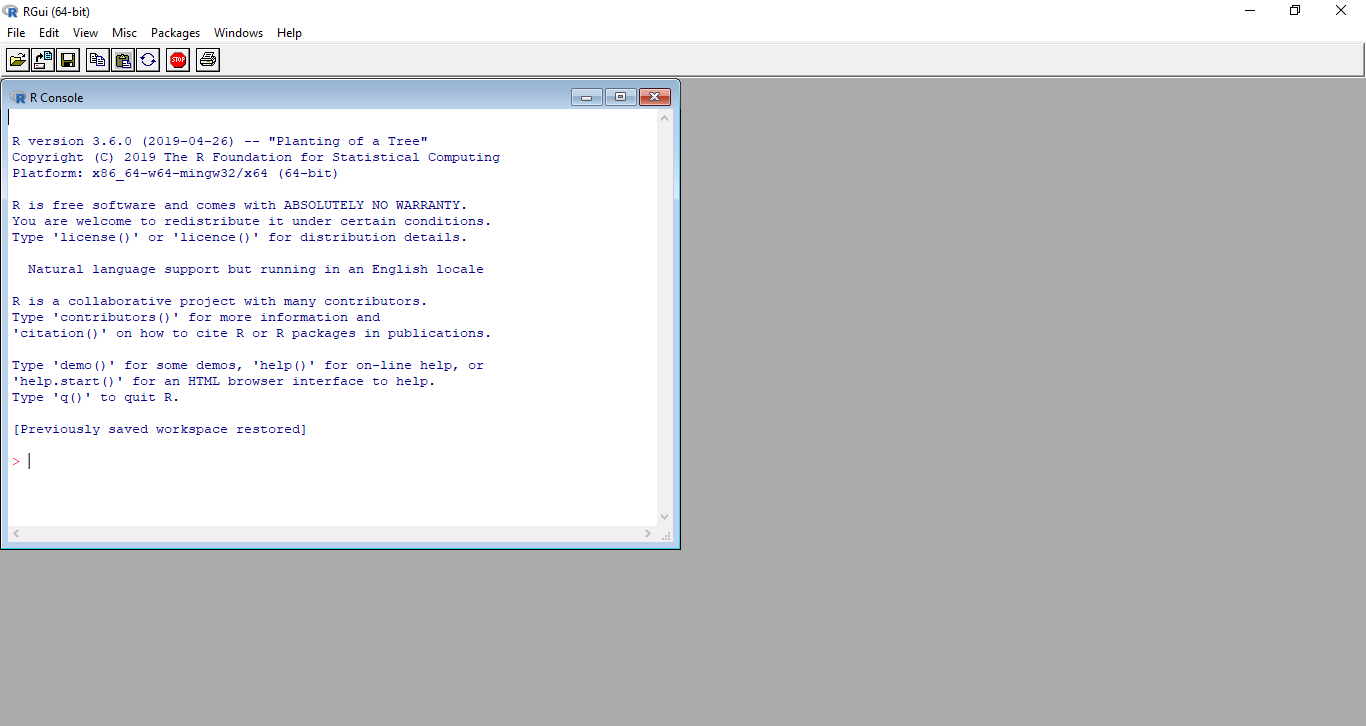
\includegraphics[width=18.97in]{RGUI} 

}

\caption{R GUI}\label{fig:unnamed-chunk-4}
\end{figure}

\hypertarget{rstudio}{%
\section{RStudio}\label{rstudio}}

Sebelum membahas lebih lanjut tentang R, sebaiknya Anda download dan install \href{https://www.rstudio.com/products/rstudio/download/}{RStudio} terlebih dahulu. RStudio adalah \emph{Integrated Development Environment} (IDE) terbaik untuk R.

\begin{figure}

{\centering 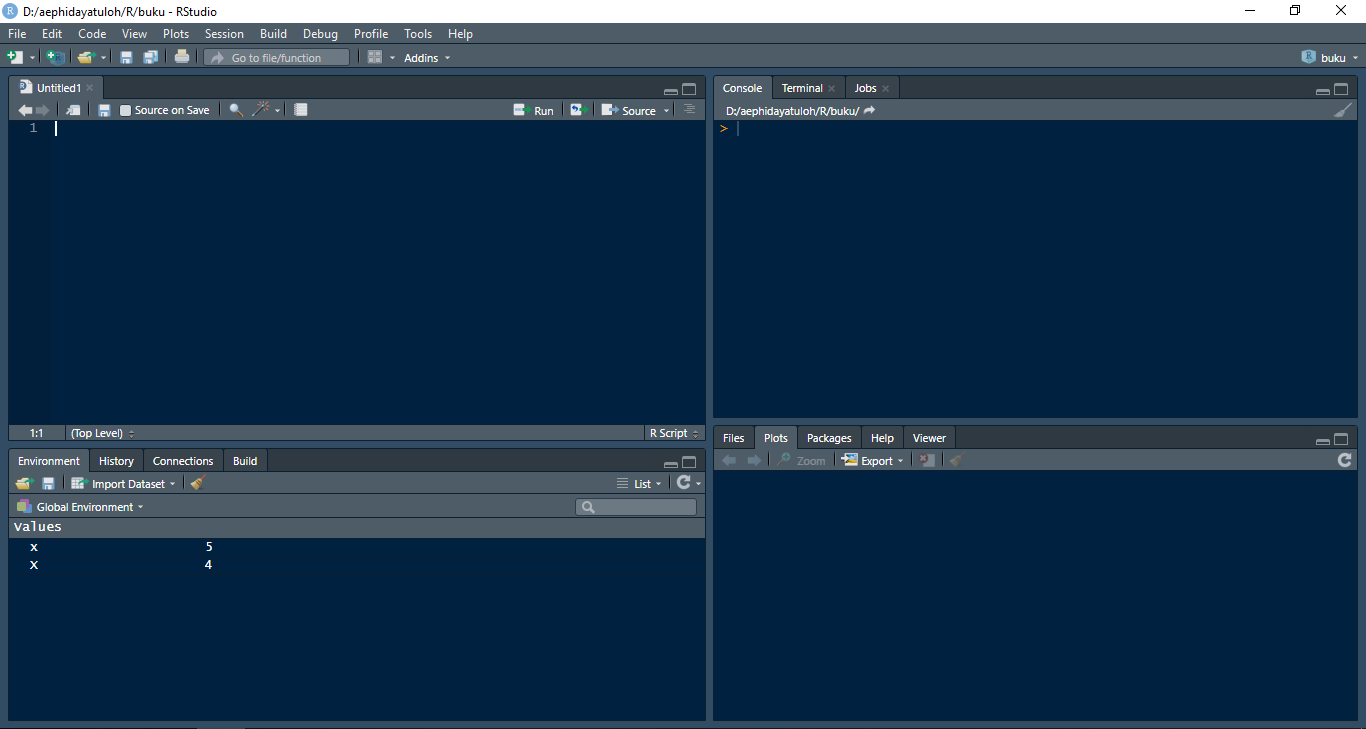
\includegraphics[width=18.97in]{rstudio2} 

}

\caption{RStudio}\label{fig:unnamed-chunk-5}
\end{figure}

\hypertarget{dasar-r}{%
\section{Dasar R}\label{dasar-r}}

Hal yang paling sederhana yang dapat dilakukan R adalah sebagai kalkulator. Coba Anda ketikan perintah di bawah ini dan tekan tombol Enter setelah selesai.

\begin{Shaded}
\begin{Highlighting}[]
\DecValTok{2} \OperatorTok{+}\StringTok{ }\DecValTok{4}
\end{Highlighting}
\end{Shaded}

Akan muncul hasil \texttt{{[}1{]}\ 6}. Hasil \texttt{{[}1{]}} menunjukkan bahwa yang ditampilkan adalah dari elemen pertama. Hal ini akan dibahas di bagian \ref{vector}.

Tanda \texttt{\textgreater{}} adalah prompt yang menunjukkan bahwa R sedang dalam posisi siap menerima perintah baru. Jika perintah belum lengkap maka akan berganti tanda \texttt{+}.

\begin{Shaded}
\begin{Highlighting}[]
\OperatorTok{>}\StringTok{ }\DecValTok{2} \OperatorTok{+}
\OperatorTok{+}
\end{Highlighting}
\end{Shaded}

Perhatikan setelah Anda tekan tombol Enter maka kursor di R yang sebelumnya \texttt{\textgreater{}} berganti \texttt{+} yang menandakan bahwa perintah belum lengkap. Maka jika Anda kembali menuliskan bilangan lain, misalkan \texttt{4} dan tekan tombol Enter maka prompt di R akan kembali menjadi \texttt{\textgreater{}} setelah menuliskan hasilnya karena perintah sudah lengkap dan selesai.

\begin{Shaded}
\begin{Highlighting}[]
\KeywordTok{print}\NormalTok{(}\StringTok{"Hello World!"}\NormalTok{)}
\end{Highlighting}
\end{Shaded}

\begin{verbatim}
## [1] "Hello World!"
\end{verbatim}

R adalah bahasa pemrograman yang \emph{case-sensitive}. Artinya perbedaan huruf kapital dan huruf kecil sangat berpengaruh.

\begin{Shaded}
\begin{Highlighting}[]
\NormalTok{a <-}\StringTok{ }\DecValTok{3}
\NormalTok{a}
\CommentTok{## [1] 3}
\end{Highlighting}
\end{Shaded}

\begin{Shaded}
\begin{Highlighting}[]
\NormalTok{A}
\CommentTok{## Error: object 'A' not found}
\end{Highlighting}
\end{Shaded}

\hypertarget{assignment}{%
\subsection{\texorpdfstring{\emph{Assignment}}{Assignment}}\label{assignment}}

Operator \emph{assignment} di R umumnya menggunakan \texttt{\textless{}-}.

\begin{Shaded}
\begin{Highlighting}[]
\NormalTok{x <-}\StringTok{ }\DecValTok{5}
\NormalTok{x}
\end{Highlighting}
\end{Shaded}

\begin{verbatim}
## [1] 5
\end{verbatim}

\begin{Shaded}
\begin{Highlighting}[]
\KeywordTok{tables}\NormalTok{(}\StringTok{"Operator Assignment"}\NormalTok{)}
\end{Highlighting}
\end{Shaded}

\begin{verbatim}
## [1] "Tabel 1: "
\end{verbatim}

\begin{longtable}[]{@{}ll@{}}
\toprule
\begin{minipage}[b]{0.24\columnwidth}\raggedright
Operator \emph{Assignment}\strut
\end{minipage} & \begin{minipage}[b]{0.70\columnwidth}\raggedright
Penjelasan\strut
\end{minipage}\tabularnewline
\midrule
\endhead
\begin{minipage}[t]{0.24\columnwidth}\raggedright
\texttt{\textless{}-}\strut
\end{minipage} & \begin{minipage}[t]{0.70\columnwidth}\raggedright
nilai dari sebelah kanan dimasukkan ke dalam objek di sebelah kiri (dapat juga menggunakan \texttt{=}).\strut
\end{minipage}\tabularnewline
\begin{minipage}[t]{0.24\columnwidth}\raggedright
\texttt{-\textgreater{}}\strut
\end{minipage} & \begin{minipage}[t]{0.70\columnwidth}\raggedright
nilai dari sebelah kiri dimasukkan ke dalam objek di sebelah kanan.\strut
\end{minipage}\tabularnewline
\begin{minipage}[t]{0.24\columnwidth}\raggedright
\texttt{\textless{}\textless{}-}\strut
\end{minipage} & \begin{minipage}[t]{0.70\columnwidth}\raggedright
nilai dari sebelah kanan dimasukkan ke dalam objek global di sebelah kiri.\strut
\end{minipage}\tabularnewline
\begin{minipage}[t]{0.24\columnwidth}\raggedright
\texttt{-\textgreater{}\textgreater{}}\strut
\end{minipage} & \begin{minipage}[t]{0.70\columnwidth}\raggedright
nilai dari sebelah kiri dimasukkan ke dalam objek global di sebelah kanan.\strut
\end{minipage}\tabularnewline
\bottomrule
\end{longtable}

Karena R adalah bahasa pemrograman yang \emph{Case Sensitive}, jadi untuk penulisan nama objek atau nilai berupa karakter sangat tergantung dari kapitalisasinya.

\begin{Shaded}
\begin{Highlighting}[]
\NormalTok{x <-}\StringTok{ }\DecValTok{5}
\NormalTok{x}
\end{Highlighting}
\end{Shaded}

\begin{verbatim}
## [1] 5
\end{verbatim}

\begin{Shaded}
\begin{Highlighting}[]
\NormalTok{X <-}\StringTok{ }\DecValTok{4}
\NormalTok{X}
\end{Highlighting}
\end{Shaded}

\begin{verbatim}
## [1] 4
\end{verbatim}

\begin{Shaded}
\begin{Highlighting}[]
\NormalTok{x <-}\StringTok{ }\DecValTok{8}
\NormalTok{x}
\end{Highlighting}
\end{Shaded}

\begin{verbatim}
## [1] 8
\end{verbatim}

Ketika menggunakan R, setiap yang ada di R disebut objek. Jenis-jenis objek dasar yang ada di R adalah vector, matriks, array, data.frame, list dan function.

\hypertarget{vector}{%
\subsection{Vector}\label{vector}}

Vector\index{vector} adalah objek paling sederhana yang ada di dalam R. Secara umum jenis data terbagi 2, yaitu numeric dan character. Ada berbagai cara untuk membuat sebuah vector di R.

\begin{enumerate}
\def\labelenumi{\arabic{enumi}.}
\tightlist
\item
  Fungsi \texttt{c()}
\end{enumerate}

Fungsi yang paling sering digunakan untuk membuat sebuah vector adalah dengan menggunakan fungsi \texttt{c()}.

\begin{Shaded}
\begin{Highlighting}[]
\NormalTok{x <-}\StringTok{ }\KeywordTok{c}\NormalTok{(}\DecValTok{2}\NormalTok{, }\DecValTok{1}\NormalTok{, }\DecValTok{5}\NormalTok{, }\DecValTok{3}\NormalTok{, }\DecValTok{1}\NormalTok{)}
\NormalTok{x}
\end{Highlighting}
\end{Shaded}

\begin{verbatim}
## [1] 2 1 5 3 1
\end{verbatim}

Pada script di atas, dibuat sebuah objek \texttt{x} berupa vector numeric. setiap elemen dipisah menggunakan tanda koma (\texttt{,}).

\begin{enumerate}
\def\labelenumi{\arabic{enumi}.}
\setcounter{enumi}{1}
\tightlist
\item
  Tanda colon (\texttt{:})
\end{enumerate}

Untuk membuat sebuah vector numeric berurutan secara meningkat atau menurun. Lihat contoh berikut ini.

\begin{Shaded}
\begin{Highlighting}[]
\CommentTok{# membuat vector numeric dengan nilai dari 1 s/d 10 secara meningkat 1}
\NormalTok{x <-}\StringTok{ }\DecValTok{1}\OperatorTok{:}\DecValTok{10} \CommentTok{# 1 sampai 10}
\NormalTok{x}
\end{Highlighting}
\end{Shaded}

\begin{verbatim}
##  [1]  1  2  3  4  5  6  7  8  9 10
\end{verbatim}

\begin{Shaded}
\begin{Highlighting}[]
\CommentTok{# membuat vector numeric dengan nilai dari 10 s/d 10 secara menurun 1}
\NormalTok{x <-}\StringTok{ }\DecValTok{10}\OperatorTok{:-}\DecValTok{10} \CommentTok{# 10 sampai -10}
\NormalTok{x}
\end{Highlighting}
\end{Shaded}

\begin{verbatim}
##  [1]  10   9   8   7   6   5   4   3   2   1   0  -1  -2  -3  -4  -5  -6
## [18]  -7  -8  -9 -10
\end{verbatim}

\begin{enumerate}
\def\labelenumi{\arabic{enumi}.}
\setcounter{enumi}{2}
\tightlist
\item
  Fungsi \texttt{seq()}
\end{enumerate}

Membuat vector berurutan dan dengan \emph{increment} tertentu.

\begin{Shaded}
\begin{Highlighting}[]
\NormalTok{x <-}\StringTok{ }\KeywordTok{seq}\NormalTok{(}\DataTypeTok{from =} \DecValTok{1}\NormalTok{, }\DataTypeTok{to =} \DecValTok{10}\NormalTok{) }\CommentTok{# 1 sampai 10 dengan increment 1 (default by = 1)}
\NormalTok{x}
\end{Highlighting}
\end{Shaded}

\begin{verbatim}
##  [1]  1  2  3  4  5  6  7  8  9 10
\end{verbatim}

\begin{Shaded}
\begin{Highlighting}[]
\NormalTok{x <-}\StringTok{ }\KeywordTok{seq}\NormalTok{(}\DataTypeTok{from =} \DecValTok{1}\NormalTok{, }\DataTypeTok{to =} \DecValTok{20}\NormalTok{, }\DataTypeTok{by =} \DecValTok{2}\NormalTok{) }\CommentTok{# 1 sampai 20 dengan increment 2}
\NormalTok{x}
\end{Highlighting}
\end{Shaded}

\begin{verbatim}
##  [1]  1  3  5  7  9 11 13 15 17 19
\end{verbatim}

\begin{Shaded}
\begin{Highlighting}[]
\NormalTok{x <-}\StringTok{ }\KeywordTok{seq}\NormalTok{(}\DataTypeTok{from =} \DecValTok{1}\NormalTok{, }\DataTypeTok{to =} \DecValTok{10}\NormalTok{, }\DataTypeTok{length.out =} \DecValTok{7}\NormalTok{) }\CommentTok{# 1 sampai 10, sebanyak 7 elemen, increment mengikuti}
\NormalTok{x}
\end{Highlighting}
\end{Shaded}

\begin{verbatim}
## [1]  1.0  2.5  4.0  5.5  7.0  8.5 10.0
\end{verbatim}

\begin{Shaded}
\begin{Highlighting}[]
\NormalTok{x <-}\StringTok{ }\KeywordTok{seq}\NormalTok{(}\DataTypeTok{from =} \DecValTok{1}\NormalTok{, }\DataTypeTok{to =} \DecValTok{10}\NormalTok{, }\DataTypeTok{along.with =} \DecValTok{1}\OperatorTok{:}\DecValTok{4}\NormalTok{) }\CommentTok{# 1 sampai 10, sebanyak elemen dari vector lain}
\NormalTok{x}
\end{Highlighting}
\end{Shaded}

\begin{verbatim}
## [1]  1  4  7 10
\end{verbatim}

\begin{enumerate}
\def\labelenumi{\arabic{enumi}.}
\setcounter{enumi}{3}
\tightlist
\item
  Mengambil satu kolom dari data.frame
\end{enumerate}

Mengambil sebuah kolom dari sebuah data.frame akan dibahas lebih jauh di bagian data.frame (bagian \ref{dataframe}). Dengan menggunakan tanda dolar \texttt{\$} dan diikuti dengan nama kolom yang akan diambil dari data.frame tersebut.

\begin{Shaded}
\begin{Highlighting}[]
\NormalTok{mtcars}\OperatorTok{$}\NormalTok{mpg}
\end{Highlighting}
\end{Shaded}

\begin{verbatim}
##  [1] 21.0 21.0 22.8 21.4 18.7 18.1 14.3 24.4 22.8 19.2 17.8 16.4 17.3 15.2
## [15] 10.4 10.4 14.7 32.4 30.4 33.9 21.5 15.5 15.2 13.3 19.2 27.3 26.0 30.4
## [29] 15.8 19.7 15.0 21.4
\end{verbatim}

\begin{quote}
Dari data.frame \texttt{mtcars} diambil kolom \texttt{mpg}
\end{quote}

\begin{enumerate}
\def\labelenumi{\arabic{enumi}.}
\setcounter{enumi}{4}
\tightlist
\item
  Fungsi \texttt{unlist()}
\end{enumerate}

Fungsi ini berguna untuk menjadikan sebuah objek list menjadi sebuah vector. Pembahasan lebih lanjut akan dibahas di bagian \ref{list}.

\begin{Shaded}
\begin{Highlighting}[]
\NormalTok{x <-}\StringTok{ }\KeywordTok{list}\NormalTok{(mtcars}\OperatorTok{$}\NormalTok{mpg, mtcars}\OperatorTok{$}\NormalTok{disp)}
\NormalTok{x}
\end{Highlighting}
\end{Shaded}

\begin{verbatim}
## [[1]]
##  [1] 21.0 21.0 22.8 21.4 18.7 18.1 14.3 24.4 22.8 19.2 17.8 16.4 17.3 15.2
## [15] 10.4 10.4 14.7 32.4 30.4 33.9 21.5 15.5 15.2 13.3 19.2 27.3 26.0 30.4
## [29] 15.8 19.7 15.0 21.4
## 
## [[2]]
##  [1] 160.0 160.0 108.0 258.0 360.0 225.0 360.0 146.7 140.8 167.6 167.6
## [12] 275.8 275.8 275.8 472.0 460.0 440.0  78.7  75.7  71.1 120.1 318.0
## [23] 304.0 350.0 400.0  79.0 120.3  95.1 351.0 145.0 301.0 121.0
\end{verbatim}

\begin{Shaded}
\begin{Highlighting}[]
\NormalTok{x <-}\StringTok{ }\KeywordTok{unlist}\NormalTok{(x)}
\NormalTok{x}
\end{Highlighting}
\end{Shaded}

\begin{verbatim}
##  [1]  21.0  21.0  22.8  21.4  18.7  18.1  14.3  24.4  22.8  19.2  17.8
## [12]  16.4  17.3  15.2  10.4  10.4  14.7  32.4  30.4  33.9  21.5  15.5
## [23]  15.2  13.3  19.2  27.3  26.0  30.4  15.8  19.7  15.0  21.4 160.0
## [34] 160.0 108.0 258.0 360.0 225.0 360.0 146.7 140.8 167.6 167.6 275.8
## [45] 275.8 275.8 472.0 460.0 440.0  78.7  75.7  71.1 120.1 318.0 304.0
## [56] 350.0 400.0  79.0 120.3  95.1 351.0 145.0 301.0 121.0
\end{verbatim}

Fungsi \texttt{unlist()} menggabungkan semua \texttt{list} menjadi sebuah vector.

\textbf{Catatan penting untuk vector}: walaupun ditampilkan ke samping, dimensi vector di R sebenarnya ke bawah. Bayangkan untuk sebuah vector seperti satu kolom di Ms Excel.

Semua contoh di atas untuk membuat vector adalah vector numeric. Vector numeric adalah vector yang semua elemennya bernilai dan bertipe numerik.

\hypertarget{vector-character}{%
\subsubsection{Vector Character}\label{vector-character}}

Vector character adalah vector yang semua elemennya bertipe character.

\begin{Shaded}
\begin{Highlighting}[]
\NormalTok{y <-}\StringTok{ }\KeywordTok{c}\NormalTok{(}\StringTok{"a"}\NormalTok{, }\StringTok{"A"}\NormalTok{, }\StringTok{"d"}\NormalTok{, }\StringTok{"c"}\NormalTok{)}
\NormalTok{y}
\end{Highlighting}
\end{Shaded}

\begin{verbatim}
## [1] "a" "A" "d" "c"
\end{verbatim}

Jika ketika membuat sebuah vector bernilai numerik namun ada satu saja elemennya bertipe character maka semua elemennya akan bertipe character.

\begin{Shaded}
\begin{Highlighting}[]
\KeywordTok{c}\NormalTok{(}\DecValTok{1}\NormalTok{, }\DecValTok{2}\NormalTok{, }\DecValTok{3}\NormalTok{, }\DecValTok{5}\NormalTok{, }\StringTok{"a"}\NormalTok{)}
\end{Highlighting}
\end{Shaded}

\begin{verbatim}
## [1] "1" "2" "3" "5" "a"
\end{verbatim}

Di R ada 2 buah vector khusus yang bertipe character, yaitu \texttt{letters} dan \texttt{LETTERS}.

\begin{Shaded}
\begin{Highlighting}[]
\NormalTok{letters}
\end{Highlighting}
\end{Shaded}

\begin{verbatim}
##  [1] "a" "b" "c" "d" "e" "f" "g" "h" "i" "j" "k" "l" "m" "n" "o" "p" "q"
## [18] "r" "s" "t" "u" "v" "w" "x" "y" "z"
\end{verbatim}

\begin{Shaded}
\begin{Highlighting}[]
\NormalTok{LETTERS}
\end{Highlighting}
\end{Shaded}

\begin{verbatim}
##  [1] "A" "B" "C" "D" "E" "F" "G" "H" "I" "J" "K" "L" "M" "N" "O" "P" "Q"
## [18] "R" "S" "T" "U" "V" "W" "X" "Y" "Z"
\end{verbatim}

Dua buah vector atau lebih dapat digabungkan dengan fungsi \texttt{c()}. Namun, jika salah satu vector bertipe character, maka vector hasil gabungan akan menjadi vector character.

\begin{Shaded}
\begin{Highlighting}[]
\KeywordTok{c}\NormalTok{(x, y)}
\end{Highlighting}
\end{Shaded}

\begin{verbatim}
##  [1] "21"    "21"    "22.8"  "21.4"  "18.7"  "18.1"  "14.3"  "24.4" 
##  [9] "22.8"  "19.2"  "17.8"  "16.4"  "17.3"  "15.2"  "10.4"  "10.4" 
## [17] "14.7"  "32.4"  "30.4"  "33.9"  "21.5"  "15.5"  "15.2"  "13.3" 
## [25] "19.2"  "27.3"  "26"    "30.4"  "15.8"  "19.7"  "15"    "21.4" 
## [33] "160"   "160"   "108"   "258"   "360"   "225"   "360"   "146.7"
## [41] "140.8" "167.6" "167.6" "275.8" "275.8" "275.8" "472"   "460"  
## [49] "440"   "78.7"  "75.7"  "71.1"  "120.1" "318"   "304"   "350"  
## [57] "400"   "79"    "120.3" "95.1"  "351"   "145"   "301"   "121"  
## [65] "a"     "A"     "d"     "c"
\end{verbatim}

\hypertarget{matriks}{%
\subsection{Matriks}\label{matriks}}

Matriks\index{matriks} adalah objek di R yang memiliki 2 dimensi, baris (\emph{row}) dan kolom (\emph{column}), dan tipe nilainya sama. Jika ketika membuat sebuah matriks elemennya memiliki minimal 1 elemen bertipe character maka seluruh matriks tersebut akan bertipe character. Membuat matriks di R menggunakan vector yang dikonversi dimensinya.

\begin{Shaded}
\begin{Highlighting}[]
\NormalTok{x <-}\StringTok{ }\NormalTok{mtcars}\OperatorTok{$}\NormalTok{mpg }\CommentTok{# vector}
\KeywordTok{length}\NormalTok{(x) }
\end{Highlighting}
\end{Shaded}

\begin{verbatim}
## [1] 32
\end{verbatim}

Karena vector \texttt{x} memmiliki 64 elemen, maka dimensi matriks yang dapat dibuat adalah 2 angka yang hasil perkaliannya menghasilkan nilai 32. Salah satunya adalah \texttt{8\ x\ 4\ =\ 32}.

\begin{Shaded}
\begin{Highlighting}[]
\NormalTok{m <-}\StringTok{ }\KeywordTok{matrix}\NormalTok{(}\DataTypeTok{data =}\NormalTok{ x, }\DataTypeTok{nrow =} \DecValTok{8}\NormalTok{, }\DataTypeTok{ncol =} \DecValTok{4}\NormalTok{, }\DataTypeTok{byrow =} \OtherTok{TRUE}\NormalTok{)}
\NormalTok{m}
\end{Highlighting}
\end{Shaded}

\begin{verbatim}
##      [,1] [,2] [,3] [,4]
## [1,] 21.0 21.0 22.8 21.4
## [2,] 18.7 18.1 14.3 24.4
## [3,] 22.8 19.2 17.8 16.4
## [4,] 17.3 15.2 10.4 10.4
## [5,] 14.7 32.4 30.4 33.9
## [6,] 21.5 15.5 15.2 13.3
## [7,] 19.2 27.3 26.0 30.4
## [8,] 15.8 19.7 15.0 21.4
\end{verbatim}

Matriks \texttt{m} adalah matriks berukuran 8x4. Argumen \texttt{byrow\ =\ TRUE} artinya matriks akan setiap elemen \texttt{x} diisikan ke \texttt{m} memenuhi baris terlebih dahulu. Jika \texttt{byrow\ =\ FALSE} maka setiap elemen \texttt{x} diisikan ke \texttt{m} memenuhi kolom terlebih dahulu.

Untuk membuat matriks dengan nilai yang sama seluruhnya, maka dapat dilakukan seperti berikut.

\begin{Shaded}
\begin{Highlighting}[]
\KeywordTok{matrix}\NormalTok{(}\DataTypeTok{data =} \DecValTok{0}\NormalTok{, }\DataTypeTok{nrow =} \DecValTok{5}\NormalTok{, }\DataTypeTok{ncol =} \DecValTok{6}\NormalTok{)}
\end{Highlighting}
\end{Shaded}

\begin{verbatim}
##      [,1] [,2] [,3] [,4] [,5] [,6]
## [1,]    0    0    0    0    0    0
## [2,]    0    0    0    0    0    0
## [3,]    0    0    0    0    0    0
## [4,]    0    0    0    0    0    0
## [5,]    0    0    0    0    0    0
\end{verbatim}

Untuk mengakses elemen dari suatu matriks, Anda dapat menggunakan indeks dari baris atau kolomnya.

\begin{Shaded}
\begin{Highlighting}[]
\CommentTok{# Mengambil elemen matriks `m` di baris 4}
\NormalTok{m[}\DecValTok{4}\NormalTok{, ]}
\end{Highlighting}
\end{Shaded}

\begin{verbatim}
## [1] 17.3 15.2 10.4 10.4
\end{verbatim}

\begin{Shaded}
\begin{Highlighting}[]
\CommentTok{# Mengambil elemen matriks `m` di kolom 3}
\NormalTok{m[, }\DecValTok{3}\NormalTok{]}
\end{Highlighting}
\end{Shaded}

\begin{verbatim}
## [1] 22.8 14.3 17.8 10.4 30.4 15.2 26.0 15.0
\end{verbatim}

\begin{Shaded}
\begin{Highlighting}[]
\CommentTok{# Mengambil elemen matriks `m` di baris 4 dan kolom 3}
\NormalTok{m[}\DecValTok{4}\NormalTok{, }\DecValTok{3}\NormalTok{]}
\end{Highlighting}
\end{Shaded}

\begin{verbatim}
## [1] 10.4
\end{verbatim}

\begin{Shaded}
\begin{Highlighting}[]
\CommentTok{# Mengambil elemen matriks `m` di baris 4 dan 6, dan kolom 3}
\NormalTok{m[}\KeywordTok{c}\NormalTok{(}\DecValTok{4}\NormalTok{, }\DecValTok{6}\NormalTok{), }\DecValTok{3}\NormalTok{]}
\end{Highlighting}
\end{Shaded}

\begin{verbatim}
## [1] 10.4 15.2
\end{verbatim}

R menyediakan sebuah fungsi yaitu \texttt{diag()} untuk mengakses nilai-nilai pada diagonal utama sebuah matriks.

\begin{Shaded}
\begin{Highlighting}[]
\KeywordTok{diag}\NormalTok{(m)}
\end{Highlighting}
\end{Shaded}

\begin{verbatim}
## [1] 21.0 18.1 17.8 10.4
\end{verbatim}

Anda juga dapat mengganti nilai dari elemen suatu matriks dengan menggunakan operator \emph{assignment}.

\begin{Shaded}
\begin{Highlighting}[]
\NormalTok{m[}\DecValTok{4}\NormalTok{, }\DecValTok{3}\NormalTok{] <-}\StringTok{ }\DecValTok{0}
\NormalTok{m[}\DecValTok{4}\NormalTok{, }\DecValTok{3}\NormalTok{]}
\end{Highlighting}
\end{Shaded}

\begin{verbatim}
## [1] 0
\end{verbatim}

\begin{Shaded}
\begin{Highlighting}[]
\NormalTok{m }\CommentTok{# perhatikan elemen di baris 4 kolom 3 sudah berubah jadi 0.0}
\end{Highlighting}
\end{Shaded}

\begin{verbatim}
##      [,1] [,2] [,3] [,4]
## [1,] 21.0 21.0 22.8 21.4
## [2,] 18.7 18.1 14.3 24.4
## [3,] 22.8 19.2 17.8 16.4
## [4,] 17.3 15.2  0.0 10.4
## [5,] 14.7 32.4 30.4 33.9
## [6,] 21.5 15.5 15.2 13.3
## [7,] 19.2 27.3 26.0 30.4
## [8,] 15.8 19.7 15.0 21.4
\end{verbatim}

\hypertarget{array}{%
\subsection{Array}\label{array}}

Array\index{array} merupakan matriks dengan dimensi lebih banyak. Jika matriks hanya mempunyai 2 dimensi, maka array dapat memiliki dimensi lebih dari 2.

\begin{figure}

{\centering 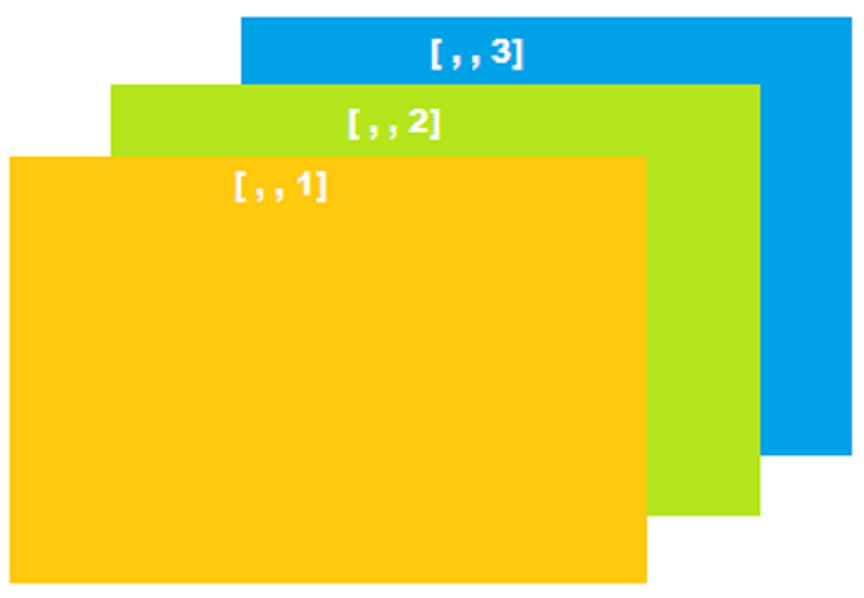
\includegraphics[width=12in]{array} 

}

\caption{Ilustrasi Array 3 dimensi}\label{fig:unnamed-chunk-30}
\end{figure}

\begin{Shaded}
\begin{Highlighting}[]
\KeywordTok{array}\NormalTok{(mtcars}\OperatorTok{$}\NormalTok{mpg, }\DataTypeTok{dim =} \KeywordTok{c}\NormalTok{(}\DecValTok{4}\NormalTok{, }\DecValTok{4}\NormalTok{, }\DecValTok{2}\NormalTok{))}
\end{Highlighting}
\end{Shaded}

\begin{verbatim}
## , , 1
## 
##      [,1] [,2] [,3] [,4]
## [1,] 21.0 18.7 22.8 17.3
## [2,] 21.0 18.1 19.2 15.2
## [3,] 22.8 14.3 17.8 10.4
## [4,] 21.4 24.4 16.4 10.4
## 
## , , 2
## 
##      [,1] [,2] [,3] [,4]
## [1,] 14.7 21.5 19.2 15.8
## [2,] 32.4 15.5 27.3 19.7
## [3,] 30.4 15.2 26.0 15.0
## [4,] 33.9 13.3 30.4 21.4
\end{verbatim}

Salah satu array yang ada setelah Anda install R adalah array \texttt{Titanic}.

\begin{Shaded}
\begin{Highlighting}[]
\NormalTok{Titanic}
\end{Highlighting}
\end{Shaded}

\begin{verbatim}
## , , Age = Child, Survived = No
## 
##       Sex
## Class  Male Female
##   1st     0      0
##   2nd     0      0
##   3rd    35     17
##   Crew    0      0
## 
## , , Age = Adult, Survived = No
## 
##       Sex
## Class  Male Female
##   1st   118      4
##   2nd   154     13
##   3rd   387     89
##   Crew  670      3
## 
## , , Age = Child, Survived = Yes
## 
##       Sex
## Class  Male Female
##   1st     5      1
##   2nd    11     13
##   3rd    13     14
##   Crew    0      0
## 
## , , Age = Adult, Survived = Yes
## 
##       Sex
## Class  Male Female
##   1st    57    140
##   2nd    14     80
##   3rd    75     76
##   Crew  192     20
\end{verbatim}

\hypertarget{dataframe}{%
\subsection{Data.frame}\label{dataframe}}

\hypertarget{list}{%
\subsection{List}\label{list}}

\hypertarget{function}{%
\subsection{Function}\label{function}}

\hypertarget{latihan}{%
\section{Latihan}\label{latihan}}

\begin{enumerate}
\def\labelenumi{\arabic{enumi}.}
\item
  Buatlah sebuah vector dengan nama \texttt{x1} yang merupakan gabungan dari kolom \texttt{drat} dan \texttt{wt} dari data.frame \texttt{mtcars}.
\item
\end{enumerate}

\hypertarget{functionandpackage}{%
\chapter{Function dan Packages}\label{functionandpackage}}

Membahas cara menggunakan fungsi yang sudah ada di R, membuat fungsi sendiri dan cara menggunakan package.

\hypertarget{externaldata}{%
\chapter{Data Eksternal}\label{externaldata}}

Membahas cara membaca data eksternal (text, cvs, Excel, database) menggunakan berbagai fungsi dan package.

Some \emph{significant} applications are demonstrated in this chapter.

\hypertarget{example-one}{%
\section{Example one}\label{example-one}}

\hypertarget{example-two}{%
\section{Example two}\label{example-two}}

\hypertarget{exploration}{%
\chapter{Eksplorasi Data}\label{exploration}}

Membahas cara eksplorasi data secara numerik maupun grafik dasar R dan visualisasinya menggunnakan ggplot2.

\hypertarget{clustering}{%
\chapter{Analisis Cluster}\label{clustering}}

Membahas secara teori dari analisis gerombol dan contoh program R pada data Iris

This is an R Markdown document. Markdown is a simple formatting syntax for authoring HTML, PDF, and MS Word documents. For more details on using R Markdown see \url{http://rmarkdown.rstudio.com}.

When you click the \textbf{Knit} button a document will be generated that includes both content as well as the output of any embedded R code chunks within the document. You can embed an R code chunk like this:

\begin{Shaded}
\begin{Highlighting}[]
\KeywordTok{summary}\NormalTok{(cars)}
\end{Highlighting}
\end{Shaded}

\begin{verbatim}
##      speed           dist       
##  Min.   : 4.0   Min.   :  2.00  
##  1st Qu.:12.0   1st Qu.: 26.00  
##  Median :15.0   Median : 36.00  
##  Mean   :15.4   Mean   : 42.98  
##  3rd Qu.:19.0   3rd Qu.: 56.00  
##  Max.   :25.0   Max.   :120.00
\end{verbatim}

\hypertarget{including-plots}{%
\section{Including Plots}\label{including-plots}}

You can also embed plots, for example:

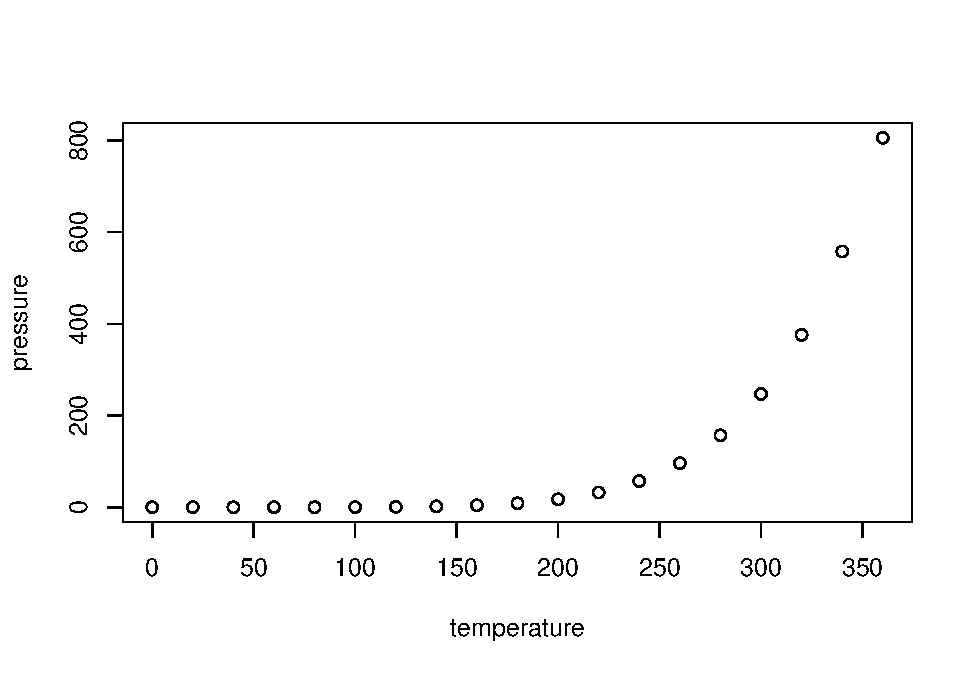
\includegraphics{buku_files/figure-latex/pressure-1.pdf}

Note that the \texttt{echo\ =\ FALSE} parameter was added to the code chunk to prevent printing of the R code that generated the plot.

\hypertarget{arules}{%
\chapter{Association Rules}\label{arules}}

Membahas teori dan pengaplikasian association rule pada data groceries.

This is an R Markdown document. Markdown is a simple formatting syntax for authoring HTML, PDF, and MS Word documents. For more details on using R Markdown see \url{http://rmarkdown.rstudio.com}.

When you click the \textbf{Knit} button a document will be generated that includes both content as well as the output of any embedded R code chunks within the document. You can embed an R code chunk like this:

\hypertarget{linearreg}{%
\chapter{Regresi Linier}\label{linearreg}}

Membahas teori (singkat) dan pengaplikasian regresi linier sederhana dan berganda pada data mtcars.

\hypertarget{logreg}{%
\chapter{Regresi Logistik Biner}\label{logreg}}

Membahas teori (singkat) dan pengaplikasian regresi logistik biner pada data .

\hypertarget{dectree}{%
\chapter{Decision Tree}\label{dectree}}

Membahas teori (singkat) Dan pengaplikasian Decision Tree pada data .

\hypertarget{custseg}{%
\chapter{Studi Kasus 1: Segmentasi Pelanggan}\label{custseg}}

Membahas Bisnis pada kasus Pengelompokan pelanggan untuk merancang program promo.

\hypertarget{mba}{%
\chapter{Studi Kasus 2: Market Basket}\label{mba}}

Membuat rules penawaran bundle produk pada kasus swalayan

\hypertarget{houseprice}{%
\chapter{Studi Kasus 3: Penentuan Harga Rumah}\label{houseprice}}

Membuat model Bisnis pada kasus penentuan harga rumah

\hypertarget{propensity}{%
\chapter{Studi Kasus 4: Propensity}\label{propensity}}

Membuat model Bisnis pada kasus penawaran promo.

\hypertarget{churn}{%
\chapter{Studi Kasus 5: Customer Churn}\label{churn}}

Membuat model Bisnis pada kasus customer churn perusahaan telco

\hypertarget{reporting}{%
\chapter{Reporting}\label{reporting}}

Membahas penggunaan R Markdown untuk reproducible report

\hypertarget{scheduler}{%
\chapter{Proses Terjadwal}\label{scheduler}}

Membahas cara menggunnakan Task Scheduler pada sistem operasi windows untuk pemrosesan program yang terjadwal

\hypertarget{shiny}{%
\chapter{Web Dashboard Interaktif}\label{shiny}}

Membahas cara pembuatan insteraktif dashboard menggunnakan R shiny dan bs4Dash

\hypertarget{scraping}{%
\chapter{Web Scraping}\label{scraping}}

Membahas cara mengambil data dari sebuah web menggunnakan package rvest

\hypertarget{interactiveviz}{%
\chapter{Visualisasi Interaktif}\label{interactiveviz}}

Membahas cara membuat grafik interaktif menggunnakan plotly dan highcharter

\bibliography{book.bib,packages.bib}


\end{document}
